% !TeX document-id = {75bba7c0-efc4-4a47-b5d0-e0b99ded06fc}
% !TEX encoding = UTF-8 Unicode
% !TeX TXS-program:compile = txs:///pdflatex/[--shell-escape]

\documentclass[a4paper]{article}

\usepackage[utf8]{inputenc}
\usepackage{erk}
\usepackage{times}
\usepackage{graphicx}
\usepackage[top=22.5mm, bottom=22.5mm, left=22.5mm, right=22.5mm]{geometry}
\usepackage[english]{babel}
\usepackage{bm, amsmath, amssymb}
\usepackage{minted, algpseudocode, algorithm}
\usepackage{hyperref}

% local definitions
\def\footnotemark{}%  to avoid footnote on cover page

\begin{document}
%make title
\title{Mandelbrot set}

\author{Daniel Silađi}

\affiliation{UP FAMNIT}

\email{E-mail: szilagyi.d@gmail.com}

\maketitle

%\thispagestyle{empty}

\begin{abstract} {}
	In this paper, we present a unified framework for rendering the Mandelbrot set. The key idea is to decouple the job-producing part (Queue) from the job-consuming part (Processor). Using this abstraction, we demonstrate how to solve the problem serially, with multiple threads, with message passing between multiple single-threaded processes (MPI), and finally with MPI and multi-threading.
	The obtained performance measurements indicate
	
	Finally, we also describe the design of a simple GUI that uses the aforementioned programs to interactively display the set.
\end{abstract}

\section{Introduction}
	The Mandelbrot set is the set of complex numbers $c$ for which the function \[f_c(z) = z^2 + c\]
	does not diverge when iterated starting from $z=0$. In other words, the set \[\{f_c^n(z) : n\in \mathbb N\}\]
	is bounded in absolute value (here, we define $f_c^1(z) = f_c(z)$ and $f_c^{n+1} (z) = f_c(f_c^n (z))$). 
	
	The graphical representation of the set can be obtained by assigning a color to each point $c$ in the complex plane, depending on whether (and how quickly) does the sequence $\{f_c^n(z)\}$ diverge. More specifically, for each pixel $(i, j)$, we can get the corresponding complex number $c$, and coloring the pixel according to the \emph{escape time} algorithm (\ref{alg:escape time}).
	
	\begin{algorithm}[h]
		\caption{Escape time} \label{alg:escape time}
		\begin{algorithmic}[1]
			\Function{Escape-Time}{$c$}
				\State $i \gets 1$
				\State $z \gets 0$
				\While{$i\leq N$ and $|c| < 2$}
					\State $z \gets z^2 + c$
					\State $i \gets i+1$
				\EndWhile
				\State \Return $i/N$
			\EndFunction
		\end{algorithmic}
	\end{algorithm}
	
	Here, $N$ is the maximum number of iterations, and the main algorithm assigns colors to individual pixels based on the \textsc{Escape-Time} value for every $c$.
	
	Since every pixel is processed independently from the others, this algorithm can easily be parallelized, and adapted to use multiple threads, processes and machines. Thus, the rest of the paper will describe the methods used for parallelization, and the measured performance results for different degrees of parallelism. 
	
	\section{Design}
	In order to parallelize our computation, we must decide on a way to distribute the work among several (abstract) workers. Assuming that we have a fixed number of workers throughout the program execution, it would be the easiest to assign exactly one region of the resulting image to each worker. This choice is reasonable, since then each worker would only need to store the data in the region it is responsible for, and nothing else. The high memory density of the data also opens room for vectorization and improved cache usage. 
	
	However, one drawback of this approach is that, due to the structure of the Mandelbrot set, and the nature of the algorithm being used, some areas of the set (particularly those inside and at the border of the set) require a much greater amount of processing than the others. Whatever fixed division of the image we impose, we risk having some workers (and thus processing power in general) unused while they are waiting for the longer-running workers to complete.
	
	Fortunately, we can mostly overcome this problem by having a larger number of regions than there are workers. This is done by prescribing a block size, and partitioning image into roughly equally-sized blocks. Still, care must be taken when choosing the block size, as it has to be small enough to ensure a balanced usage of all workers, but at the same time, large enough not to spend most of the CPU time on worker communication and organization overhead.
	
	This design decision implies that we should design our program around a job queue, and possibly multiple workers that fetch jobs from that queue. At the end, the escape-times are submitted back to the ``owner'' of the queue, which will reconstruct the wanted image from the blocks. Further consideration of this design revealed that a lot of code can be reused between the serial and all variants of the parallel implementations of the algorithm (\ref{alg:basic algorithm}) -- enough to derive (in the object-oriented sense) all of them from a single basic algorithm, and two data structures, the \emph{Queue} (to avoid confusion, we will always write it with a capital letter, and denote the usual FIFO data structure with a small letter) and the \emph{Processor}. 
	
	\begin{algorithm}
		\caption{Basic algorithm} \label{alg:basic algorithm}
		\begin{algorithmic}[1]
			\Procedure{Main}{processor, queue}
				\State queue.init()
				\State processor.init(queue)
				\State processor.process\_queue()
				\State processor.finalize()
			\EndProcedure
		\end{algorithmic}
	\end{algorithm}	
	
	\section{Problem description}
	Before describing the Queue and Processor interfaces and their implementations, we will first describe the problems these interfaces are designed to solve. To do that, we will specify how exactly should each of the 4 execution modes of the program behave.
	
	\begin{description}
		\item[Serial mode:] This is the most basic mode, that uses a single thread for everything. First should load the job specification (the resolution of the image being rendered, and its position and dimensions in the Mandelbrot-space). Then, it should split the job into a number of smaller jobs (for compatibility with other modes), and place them into a queue. Finally, it should process each job, and render the resulting image.
		\item[Parallel (multi-threaded) mode:] Here, the job loading and splitting part is the same as in the serial mode. However, once the job queue is filled, it should spawn some worker threads and coordinate job division between them. After the worker threads have finished their work, they should send back their chunks to the main thread, which will reconstruct the final image.
		\item[Distributed (MPI) mode:] In this mode, we have to have at least two processes running, the server and at least one worker. The server handles the job loading and splitting part, and waits for job requests from the workers. The workers should in turn request jobs from the server, and process them. When there are no more jobs left to process, the workers should send back their chunks to the server, which will use them to reconstruct the final image. Here, we see that we didn't specify the type of the workers -- it turns out that with some careful design, we can get both serial and parallel workers ``for free'', by reusing most of the code for the serial and parallel modes.
	\end{description}
	
	\section{The Processor and Queue interfaces}
	From the previous section we can see that each execution mode has roughly two independent parts: 
	\begin{description}
		\item[The Queue,] responsible for containing the actual job queue, as well as the supporting operations of loading the job specification, generating the jobs, acting as a sink for the processed jobs (and reassembling them later), and
		\item[The Processor,] responsible for fetching jobs from the queue, processing them, and submitting the results back to the Queue.
	\end{description}
	
	These parts are implemented as abstract classes with the following interfaces
	
	\begin{minted}[tabsize=4, breaklines=true]{C++}
struct Queue {
	virtual void push(Job job);
	virtual void pop();
	virtual Job front();
	virtual bool empty();
	virtual void submit_result( JobResult&& result );
	virtual void finalize() {}
	virtual ~Queue() {}
};
	\end{minted}
	
	\begin{minted}[tabsize=4, breaklines=true]{C++}
struct Processor {
	Queue *queue;
	Processor(Queue *queue) : queue(queue) {}
	virtual void process(Job& job);
	virtual void process_queue() {
		while (!queue->empty()) {
			Job&& job = queue->front();
			process(job);
			queue->pop();
		}
	}
	virtual void finalize() {}
	virtual ~Processor() {
		delete queue;
	}
};
	\end{minted}
	
	In order to add a new Queue or Processor, one just has to implement the unimplemented functions in these interfaces. In our case, we can get away with 2 types of Queues and 3 types of Processors, that get dispatched at runtime, based on the command line arguments given to the program. Their details follow.
	
	\subsection{Queues}
	The two types of Queues that were implemented were the Local Queue, and the MPI Virtual Queue.
	\begin{description}
		\item[Local Queue:] The Local Queue is a simple wrapper for a built-in queue. It is designed to be used in the serial, parallel, and distributed server modes. Therefore, it is designed to load the job specification from disk, handle job splitting, and reconstruct the result. Notably, it is threading-agnostic, and that part is handled by the appropriate processor.
		\item[MPI Virtual Queue:] Far more interesting is the MPI Virtual Queue, as it was designed to be a drop-in replacement for the Local Queue used by the serial and parallel Processors. In itself, it contains the MPI context, that is used for obtaining jobs from the MPI server. Naturally, the \texttt{submit\_result} function is also implemented on top of MPI. Similarly to the Local Queue, this Queue is also threading-agnostic. These design choices greatly simplified the implementation, as, on one hand the Queue doesn't have to be aware of the threadedness of the worker, and, on the other hand, the worker doesn't have to care about the internal implementation of the Queue it is using.
	\end{description}
	
	\subsection{Processors}
	The Processors are actually the place where most of the work is done. Still, their implementation is fairly straightforward, as two (the Singlethreaded Worker, and the MPI Server) out of three only need to implement the \texttt{process} function, while the remaining (Multithreaded Worker) had to implement the \texttt{process\_queue} function, as well. Their full descriptions follow.
	\begin{description}
		\item[Singlethreaded Worker] As expected, this is the most basic form of a Processor. It really only contains some glue code between the other components of the program.
		\item[Multithreaded Worker] This Processor takes care of spawning an appropriate number of worker threads, fetching the jobs from the Queue, and serving them to the worker threads in a thread-safe manner, and collecting the results from the threads, again in a thread-safe manner. Its main components are two lock-free queues ($Q_\text{master-slave}$ and $Q_\text{slave-master}$), that are used for bidirectional communication between the master and the slave (worker) threads. Additionally, a condition variable is used to sleep the master thread while it is waiting for job requests from workers. The important parts of its code is listed below, as a part of algorithms \ref{alg:multithreaded worker} and \ref{alg:multithreaded worker function} (square brackets denote atomic operations).
		
		\begin{algorithm}
			\caption{Multithreaded queue processing} \label{alg:multithreaded worker}
			\begin{algorithmic}[1]
				\Procedure{process\_queue}{}
					\State [ $n_\text{idle} \gets 0$ ]
					\State spawn $k$ worker threads
					\While{there are jobs in the main queue}
						\State wait for the condition variable to wake the thread up
						\State $[m \gets n_\text{idle}]$
						\State fetch $m$ jobs from the main queue, and push them into $Q_\text{master-slave}$
					\EndWhile
					\State result\_storage $\gets \emptyset$
					\While{ $|$result\_storage$|$ $<$ number of jobs fetched from the main queue}
						\State fetch as many jobs as possible from $Q_\text{slave-master}$
						\State yield the execution back to the thread scheduler
					\EndWhile
					\State everything\_done $\gets$ true
					\State join the $k$ worker threads
				\EndProcedure
			\end{algorithmic}
		\end{algorithm}	
		
		\begin{algorithm}
			\caption{Multithreaded worker function} \label{alg:multithreaded worker function}
			\begin{algorithmic}[1]
				\Procedure{worker\_function}{}
					\State [ $n_\text{idle} \gets n_\text{idle} + 1$ ]
					\While{not everything\_done}
						\State wake up the master thread using the condition variable
						\While{possible, atomically take a job $j$ from $Q_\text{master-slave}$}
							\State [ $n_\text{idle} \gets n_\text{idle} - 1$ ]
							\State process $j$, and push the result to $Q_\text{slave-master}$
							\State [ $n_\text{idle} \gets n_\text{idle} + 1$ ]
						\EndWhile
						\State yield to the scheduler
					\EndWhile
				\EndProcedure
			\end{algorithmic}
		\end{algorithm}
	
		Essentially, the correctness of the algorithms is guaranteed by the lock-free properties of the two queues used. First of all, assume that the scheduling is fair, in the sense that after any time $t$, every thread will be scheduled. Then, we can guarantee that the master thread will never be stuck waiting for the condition variable, as, eventually, a worker thread will be scheduled, become idle, and wake up the master thread. The $n_\text{idle}$ is just an approximation to the number of workers that are available for doing some work. The only important part is that we do not want it to be zero, but, by design, if it is, the workers will empty their queue, and become idle.
		
		The worker code is also correct, since, when we say that everything is done, the master really has received all the job results, so it is safe to quit the worker thread. The only concern here is that a worker might never grab a job from its queue time (before other threads take it) -- but, this can be addressed by increasing the individual job size, so that workers can not process them too quickly one after another. Either way, if the jobs are being processed by any worker (and they are), we have no problems!
		
		\item[MPI server] The MPI server can only be used in conjunction with a Local Queue. It sets up the MPI context, and broadcasts its rank to the rest of the workers (via MPI Virtual Queues). Then, it waits for the job requests, and responds with jobs from its own queue. Given that it is single-threaded, its implementation is relatively straightforward.
	\end{description}

	\section{Technical remarks}
	The program was implemented in C++, using a few helper libraries. As an academic exercise, some parts of the program depend on features from the draft C++17 standard, however they are mostly syntactical sugar, by their nature. Moreover, the program is designed to be as portable as possible, and can be run on both Windows and Linux, provided that they have a recent-enough C++ compiler. Most of the program configuration (including the job specification) is loaded from a JSON file, and the output is written to a Portable PixMap (PPM) image, since it is the simplest image format which is supported by mainstream image viewers.
	
	A technically interesting part of the implementation was implementing a modern object-oriented and templated wrapper for the C-language MPI bindings. Using template metaprogramming, one is able to send and receive arbitrary datatypes using generic \texttt{Send} and \texttt{Recv} functions. This eliminates the tedium of manually explaining the data structure layout to MPI.
	
	Furthermore, the design of the program was decoupled as much as possible, so aside from the aforementioned Processor and Queue abstractions, other components such as the escape-time algorithm and the MPI bindings are all replaceable, as long as they implement the same interface. For example, one could replace the escape-time algorithm with a completely different iterating function, or modify the MPI bindings to use a more robust serialization method.
	
	Finally, a thin interactive OpenGL GUI layer is implemented in Python, as well. It supports panning and zooming around the set, with live recalculation when the zoom-level exceeds 1, that is, when the GPU would need to upsample the image beyond its natural resolution. In order to be as portable as possible, no advanced inter-process communication is performed, instead, the worker program is invoked using Python's standardized subprocess library. As an optimization, the image is always rendered with a buffer area around the current screen viewport, so that the user can pan around without triggering a recalculation.
	
	\section{Results}
	The program was evaluated on a 4-node cluster, where each node has two 4-core Intel Xeon E5345 processors. The parameters that were varied were the number of nodes (1 to 4), number of processes per node (1 to 8), and the number of threads per process (1 to 8). For each triple of parameters, the measurement was performed 5 times, and the average of those measurements is taken as the result. This is a reasonable choice, since the standard deviations were relatively small (50 - 100ms) compared to the total runtimes (6 - 140s). The results are displayed as speedups over the baseline, which is taken to be the runtime of a single-threaded program on a single processor. On figures \ref{fig: 1 node speedup} to \ref{fig: 4 node speedup}, we can see the speedups for various numbers of nodes used in the computation.  
	
	\begin{figure}
		\centering
		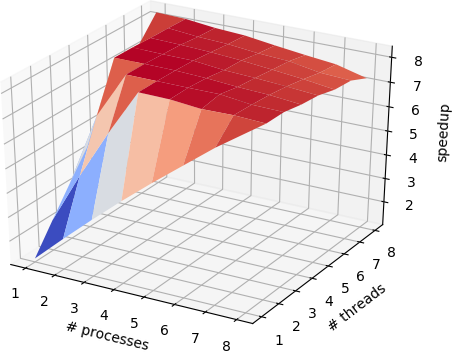
\includegraphics[width=0.8\linewidth]{1node.png}
		\caption{Speedup with 1 node}
		\label{fig: 1 node speedup}
	\end{figure}

	\begin{figure}
		\centering
		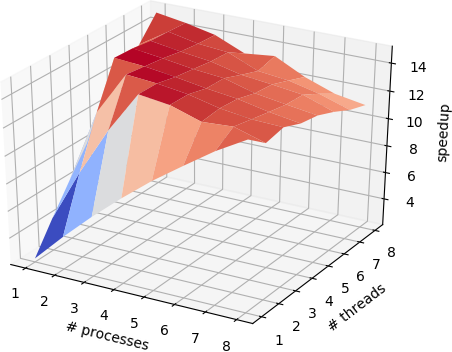
\includegraphics[width=0.8\linewidth]{2node.png}
		\caption{Speedup with 2 nodes}
		\label{fig: 2 node speedup}
	\end{figure}

	\begin{figure}
		\centering
		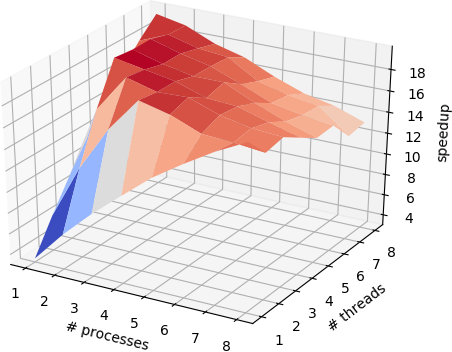
\includegraphics[width=0.8\linewidth]{3node.png}
		\caption{Speedup with 3 nodes}
		\label{fig: 3 node speedup}
	\end{figure}

	\begin{figure}
		\centering
		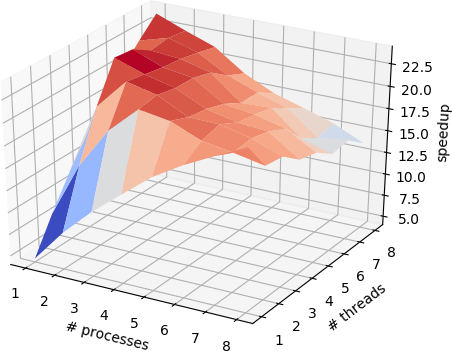
\includegraphics[width=0.8\linewidth]{4node.png}
		\caption{Speedup with 4 nodes}
		\label{fig: 4 node speedup}
	\end{figure}
	
	\section{Conclusion}
	As can be seen from the results, the presented algorithm works the best when there is only 1 process per node, that uses all hardware threads that are available, by itself. Since the problem is computationally-bound, we see that there is no benefit of using more cores then there are available on a node, and we can see from figure \ref{fig: 4 node speedup} that core oversubscription can result in up to 50\% performance degradation. We can also see that we get diminishing returns from increasing the number of nodes. This is most likely due to Amdahl's law, and can be remedied by reducing the communication overhead between nodes -- e.g. by increasing the MPI Virtual Queue buffer size.
	
	To sum up, the presented method is appropriate for rendering the Mandelbrot set at very high resolutions. Using the best practices from software engineering, a simple framework was developed, upon which robust serial, parallel and distributed backends were built.
	
\end{document}
